\documentclass[14pt]{extarticle}
\usepackage[T2A]{fontenc}
\usepackage[english, russian]{babel}
\usepackage[left=20mm, right=10mm, top=20mm, bottom=20mm]{geometry}
\usepackage{graphicx}
\usepackage{titlesec}
\usepackage{array}
\usepackage{wrapfig}
\usepackage{color, colortbl}
\usepackage[colorlinks=true,linkcolor=cyan,unicode=true]{hyperref}
\usepackage{mathtools}
\usepackage{setspace}
\usepackage{tabularx}
\usepackage{svg}
 
\newcommand\ddformula[1]{\displaystyle #1}
 
\titleformat{\section}
  {\normalfont\fontsize{14}{16}\bfseries}{\thesection}{0.5em}{}
 
\begin{document}
    \begin{minipage}{0.5\textwidth}
        \begin{center}
            \begin{small}
                \textsf{\textbf{Университет ИТМО}} \\
                \textsf{\textbf{Физико-технический мегафакультет}} \\
                \textsf{\textbf{Физический факультет}}
            \end{small}
        \end{center}
    \end{minipage}
    \hfill
    \begin{minipage}{0.4\textwidth}
        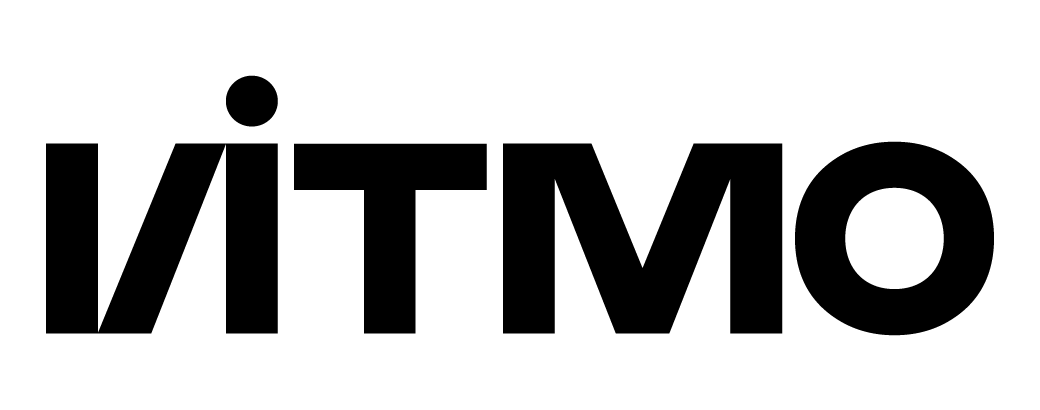
\includegraphics[height=2.5cm]{img/itmo.png}
    \end{minipage}
    \hrule
    \vspace{8mm}
    \begin{minipage}{0.4\textwidth}
        Группа: P3215 \\ % ГРУППА
        Студент: Барсуков М.А. \\ % СТУДЕНТ
        Преподаватель: Смирнов А.В % ПРЕПОД
    \end{minipage}
    \hfill
    \begin{minipage}{0.4\textwidth}
        К работе допущен: \\
        Работа выполнена: \\
        Отчёт принят: 
    \end{minipage}
    \vspace{8mm}
    \begin{center}
        \begin{Large}
            \textbf{Рабочий протокол и отчёт по лабораторной работе №3.10} \\ % УКАЗАТЬ НОМЕР ЛАБЫ
            Изучение свободных затухающих электромагнитных колебаний % УКАЗАТЬ НАЗВАНИЕ ЛАБЫ
        \end{Large}
    \end{center}
    \vspace{8mm}
 
    \section{Цель работы}
    Изучение основных характеристик свободных затухающих колебаний
    
    \section{Задачи, решаемые при выполнении работы}
    \begin{enumerate}
        \item Изучить период колебаний в контуре с разными сопротивлениями
        \item Вычислить критическое сопротивление
        \item Сравнить слабозатухающие и быстрозатухающие колебания
    \end{enumerate}
    
    \section{Объект исследования}
    Объектом исследования являются свободные затухающие колебания напряжения.

    \section{Метод экспериментального исследования}
    Получение экспериментальных значений амплитуды выходного напряжения при разных значениях частоты генератора.
    
    \section{Рабочие формулы и исходные данные}
    \textbf{Ёмкости конденсаторов} \\
    $C_1 = 0.022 \text{мкФ} \pm 10\%$ \\
    $C_2 = 0.033 \text{мкФ} \pm 10\%$ \\
    $C_3 = 0.047 \text{мкФ} \pm 10\%$ \\
    $C_4 = 0.47 \text{мкФ} \pm 10\%$ \\
    \vspace*{2mm} \\
    $L = 10 \text{мГн}$ \\
    \textbf{Логарифмический декремент затухания} \\
    \begin{equation*}
        \lambda = \frac{1}{n}\ln{\frac{U_i}{U_{i+n}}}
    \end{equation*}
    - через амплитуду колебаний напряжения
    \begin{equation*}
        \lambda = \beta T = \frac{R}{L}\frac{\pi}{\sqrt{\frac{1}{LC} - \frac{R^2}{4L^2}}}
    \end{equation*}
    - через параметры элементов контура\\
    Полное сопротивление контура:
    \begin{equation*}
        R = R_M + R_0
    \end{equation*}
    Собственное сопротивление контура:
    \begin{equation*}
        R_0 = -R_M|_{\lambda = 0}
    \end{equation*}
    Добротность контура:
    \begin{equation*}
        Q = \frac{2\pi}{1 - e^{-2\lambda}}
    \end{equation*}
    Критическое сопротивление контура:
    \begin{equation*}
        R_{\text{крит}} = 2\sqrt{\frac{L}{C}}
    \end{equation*}
    Теоретическое значение периода:
    \begin{equation*}
        T = 2\pi\sqrt{LC}
    \end{equation*}
    
    \newpage
    \section{Измерительные приборы}

    \begin{tabular}{ |m{0.7cm}|m{6cm}|m{3cm}|m{3.5cm}|m{3.5cm}| }
        \hline
        № п/п & Наименование & Тип прибора & Используемы диапазон & Погрешность прибора \\\hline
        1  & Блок генератора напряжений ГН1 & электронный & настраиваемый  & настраиваемый \\\hline
        2  & Осциллограф ОЦЛ2 & электронный & настраиваемый  & настраиваемый \\\hline
        3  & Стенд с объектом исследования С3-ЭМ01 & электронный & -  & - \\\hline
        4  & Проводники Ш4/Ш2 (4 шт), Ш2/Ш2 (3 шт), 2Ш4/BNC (2 шт) & электронный & -  & - \\\hline
    \end{tabular}
    \vspace*{5mm}\\

    \begin{figure}[h!]
        \centering
        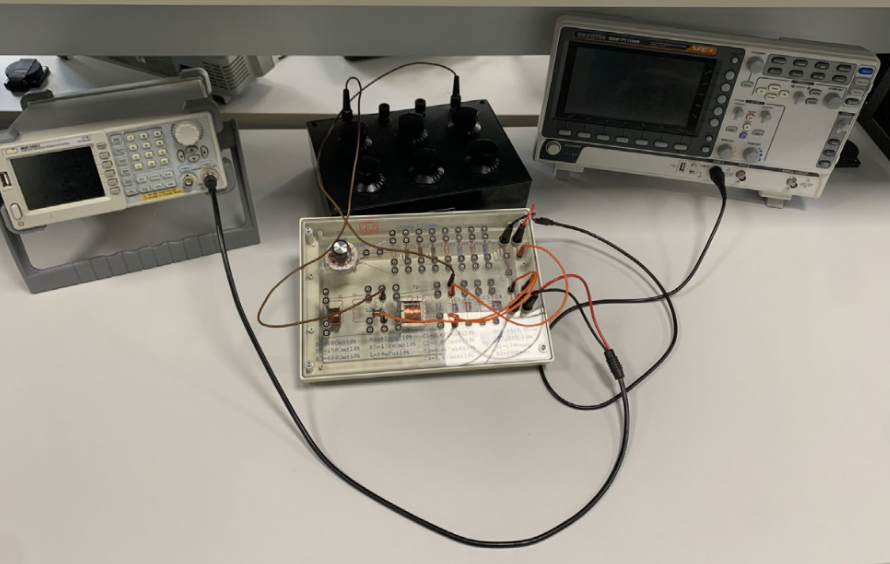
\includegraphics[height=11cm]{img/tech.png}
        \caption{Общий вид установки}
    \end{figure}
    
    \newpage
    \section{Схема установки}
    \begin{figure}[h!]
        \centering
        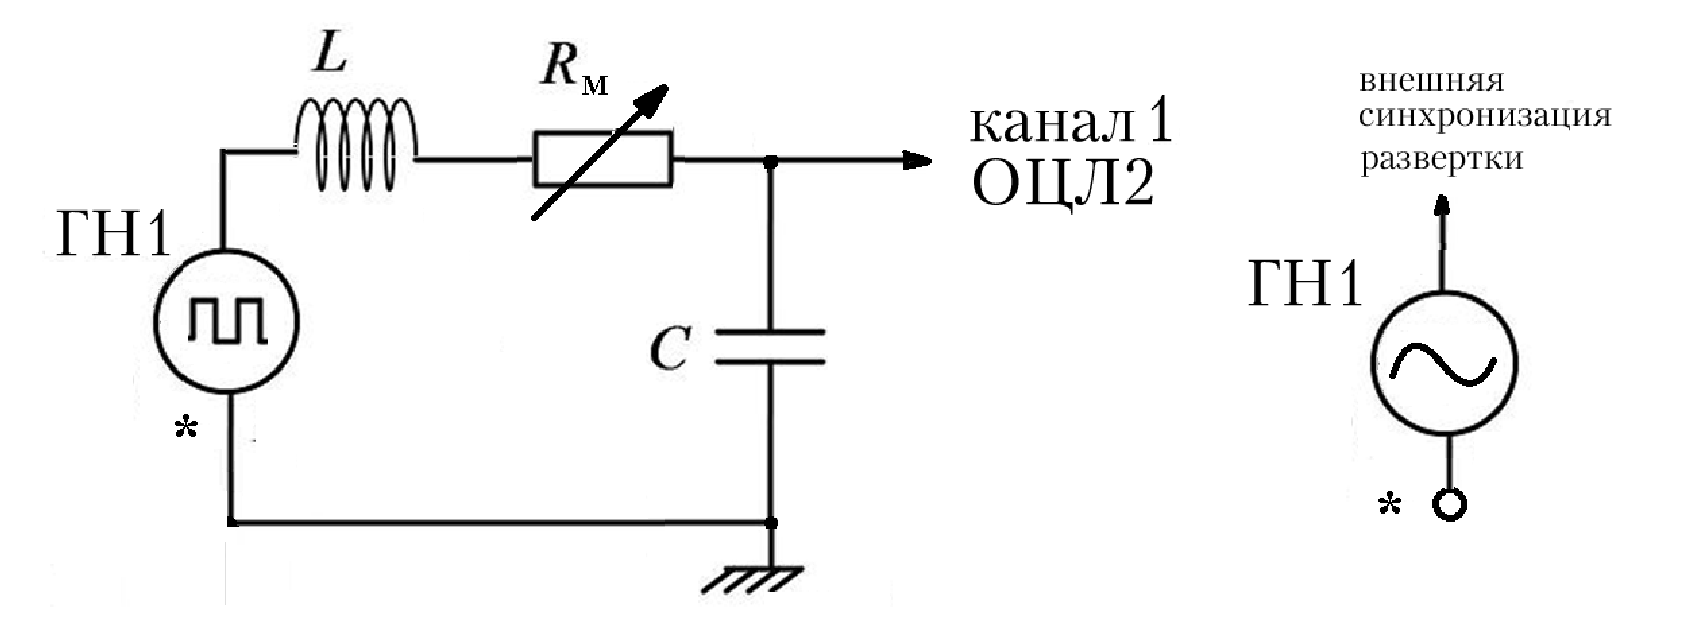
\includegraphics[height=5cm]{img/scheme1.png}
        \caption{Рабочая схема. Первый случай}
    \end{figure}
    \begin{figure}[h!]
        \centering
        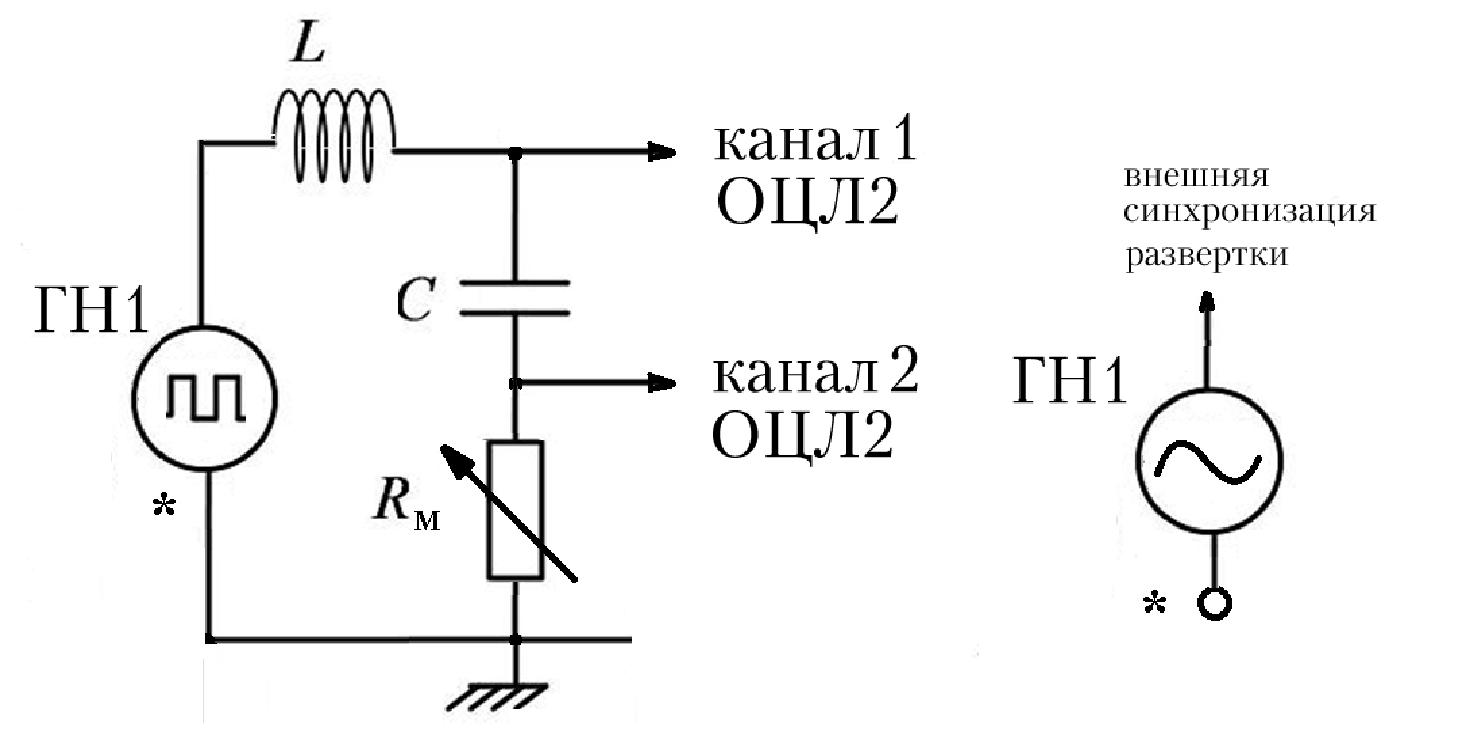
\includegraphics[height=5cm]{img/scheme2.png}
        \caption{Рабочая схема. Второй случай}
    \end{figure}

    \newpage
    \section{Результаты прямых измерений}
    \begin{tabularx}{\textwidth}{|X|X|X|X|X|}
        \hline
        $R_M$, Ом & $T$, мс & $2U_i$, дел & $2U_{i+n}$, дел & $n$ \\\hline
        0  & 87,67 & 5,34 & 1,9  & 3 \\\hline
        10 &    87,67 & 5    & 1,54 & 3 \\\hline
        20 & 87,67 & 4,68 & 1,28 & 3 \\\hline
        30 & 87,67 & 4,48 & 1,1  & 3 \\\hline
        40 & 87,67 & 4,2  & 0,92 & 3 \\\hline
        50 & 87,67 & 4,02 & 0,78 & 3 \\\hline
        60 & 87,67 & 3,76 & 0,64 & 3 \\\hline
        70 & 87,67 & 3,36 & 0,52 & 3 \\\hline
        80 & 87,67 & 3,02 & 0,4  & 3 \\\hline
        
    \end{tabularx}
    \vspace*{5mm}\\
    \begin{tabularx}{\textwidth}{|X|X|X|X|}
        \hline
        $C$, мкФ & $T_{\text{эксп}}$, мс & $T_{\text{теор}}$, мс & $\delta T$, \% \\\hline
        0,022 & 0,088 & 0,093194699 & 5,574 \\\hline
        0,033 & 0,108 & 0,114139729 & 5,379 \\\hline
        0,047 & 0,132 & 0,136216211 & 3,095 \\\hline
        0,47  & 0,422 & 0,430753483 & 2,032 \\\hline
    \end{tabularx}

    \newpage
    \section{Расчёт результатов косвенных измерений}
    Аппроксимирующая прямая (найдена с помощью метода наименьших квадратов):
    \begin{equation*}
        \lambda(R) = 0.004R + 0.348
    \end{equation*}
    Точка пересечения с осью абцисс: $R = -87 \Rightarrow R_0 = 87$, т.к. $R_0 = -R_M|_{\lambda = 0}$
    \begin{tabularx}{\textwidth}{|X|X|X|X|}
        \hline
        $\lambda$ & $Q$ & $R$ & $L$ \\\hline
        0,344457256 & 12,61989968 & 87  & 10,717475   \\\hline
        0,392551832 & 11,55151081 & 97  & 10,54973961 \\\hline
        0,432146011 & 10,85834724 & 107  & 10,83348099 \\\hline
        0,468104289 & 10,33608496 & 117 & 11,24513653 \\\hline
        0,506155378 & 9,869574981 & 127 & 11,50840932 \\\hline
        0,546581087 & 9,450601697 & 137 & 11,63553916 \\\hline
        0,590235353 & 9,068400711 & 147 & 11,61757393 \\\hline
        0,621955814 & 8,827853501 & 157 & 12,05159716 \\\hline
        0,673849188 & 8,488928227 & 167 & 11,71604632 \\\hline
    \end{tabularx}
    \vspace*{3mm}\\
    $L_{\text{ср}} = 11.319$ мГн\\
    Экспериментальный $R_{\text{крит}} = 1000$ Ом \\
    Полное сопротивление $R_{\text{крит}} = 1087$ Ом \\
    Теоретическое значение (при $L = 10$ мГн): $R_{\text{крит}} = 1348.3997$ Ом \\

    \section{Расчёт погрешностей изменений}
    Погрешность $L_{cp}$:
    \begin{equation*}
        S_{\bar{x}} = \sqrt{\frac{ \sum_{i = 1}^{n} (x_i - \bar{x})^2 }{n(n - 1)}} = 0,171364634
    \end{equation*}
    \begin{equation*}
        SE_{\bar{x}} = \frac{S_{\bar{x}}}{\sqrt{n}} = 0,057121545
    \end{equation*}
    
    \newpage
    \section{Графики}
    \begin{figure}[h!]
        \centering
        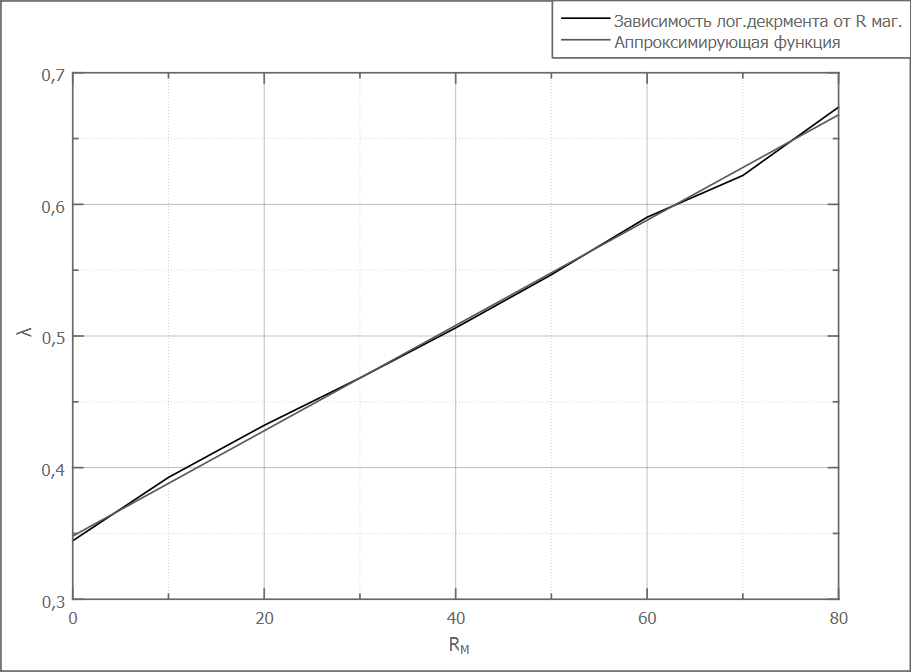
\includegraphics[height=13cm]{img/plot.png}
        \caption{График зависимости логарифмического декремента $\lambda$ от сопротивления магазина $R_M$}
    \end{figure}
    \newpage
    \begin{figure}[h!]
        \centering
        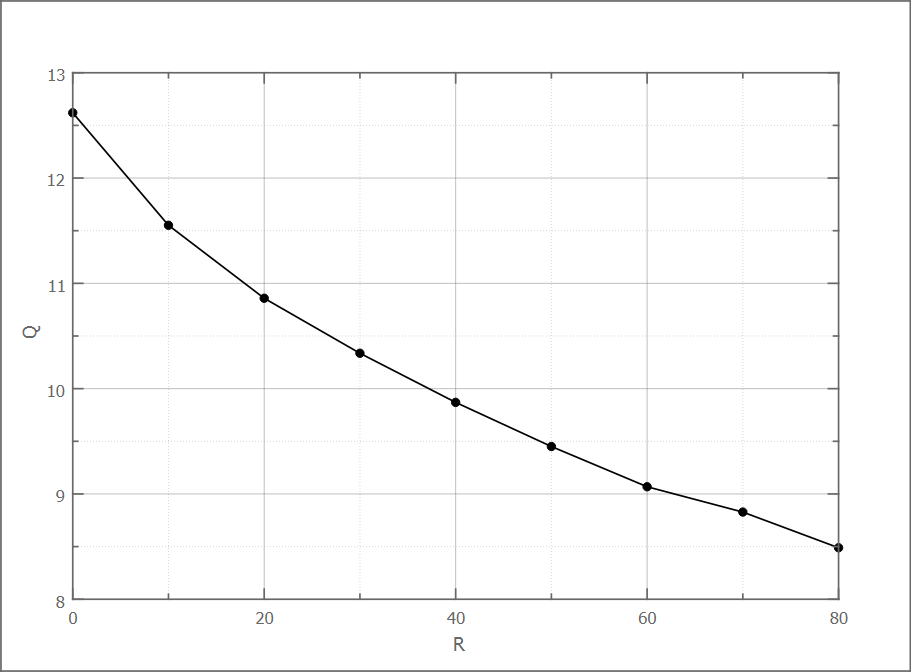
\includegraphics[height=13cm]{img/plot2.png}
        \caption{График зависимости добротности контура от сопротивления контура}
    \end{figure}
    \newpage
    \begin{figure}[h!]
        \centering
        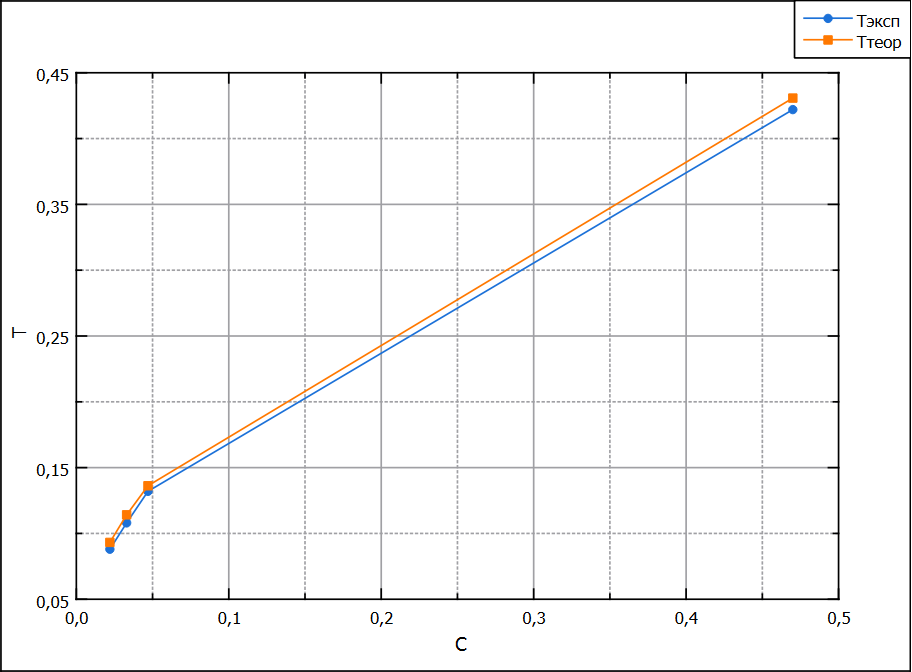
\includegraphics[height=13cm]{img/plot3.png}
        \caption{Графики зависимости $T_\text{эксп}$ и $T_\text{теор}$ от ёмкости конденсатора}
    \end{figure}

    \newpage
    \section{Окончательные результаты}
    Индуктивность катушки $L_{\text{ср}} = 11,319$ мГн \\
    Сопротивление контура $R_0 = 87$ Ом \\
    Экспериментальное критическое сопротивление контура $R_{\text{крит}} = 1087$ Ом \\
    Теоретическое критическое сопротивление контура $R_{\text{крит}} = 1348.3997$ Ом 
    
    \section{Вывод и анализ результатов}
    В рамках лабораторной работы были изучены ключевые характеристики свободных затухающих колебаний. В ходе экспериментов было установлено, что логарифмический декремент возрастает пропорционально увеличению сопротивления в контуре. Графические данные наглядно подтвердили эту зависимость, что является важным результатом. \\

    \noindent Кроме того, было выявлено, что добротность контура снижается при увеличении сопротивления, что указывает на обратную пропорциональность между этими величинами. Период колебаний, как показали исследования, увеличивается при возрастании емкости конденсатора, что соответствует теоретическим предсказаниям.\\

    \noindent Экспериментально было определено значение сопротивления, при котором разряд конденсатора перестает быть периодическим. Этот критический показатель также совпадает с теоретическими расчетами, что подтверждает правильность выполнения лабораторной работы и достоверность полученных данных.\\

    \clearpage
    \begin{figure}[h]
        \center{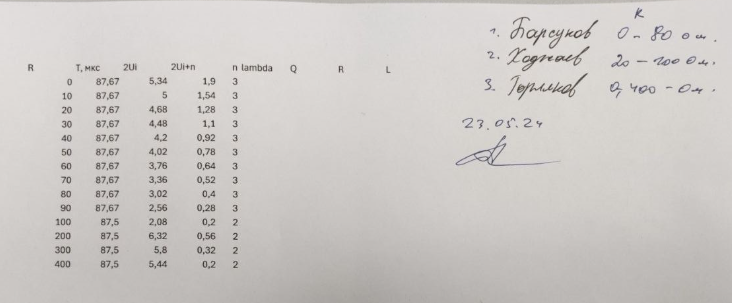
\includegraphics[width=1\linewidth]{img/sign1.png}}
    \end{figure}
    \begin{figure}[h]
        \center{
        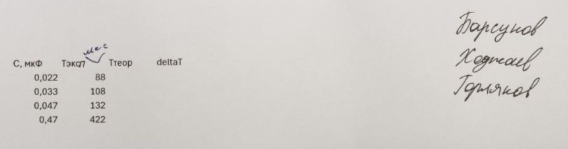
\includegraphics[width=1\linewidth]{img/sign2.png}
        \caption{Результаты измерений}
        }
    \end{figure}
\end{document}
